\documentclass{article}
\usepackage[utf8]{inputenc}
\usepackage{graphicx}

\title{ApexDatabase}
\author{itsmeakil707 }
\date{November 2019}

\begin{document}

\title{Laporan Apex Oracle}
\author{Akil Munawwar \\ D4 TI 1B \\ 1184041}
\maketitle

\section{Langkah Membuat Workspace}
\begin{enumerate}
    \item Disini kita tidak memakai apex offline, melainkan apex online
    \item Buka aplikasi nya di https://apex.oracle.com/en/learn/getting-started/
    \begin{figure}[!htbp]
        \centering
        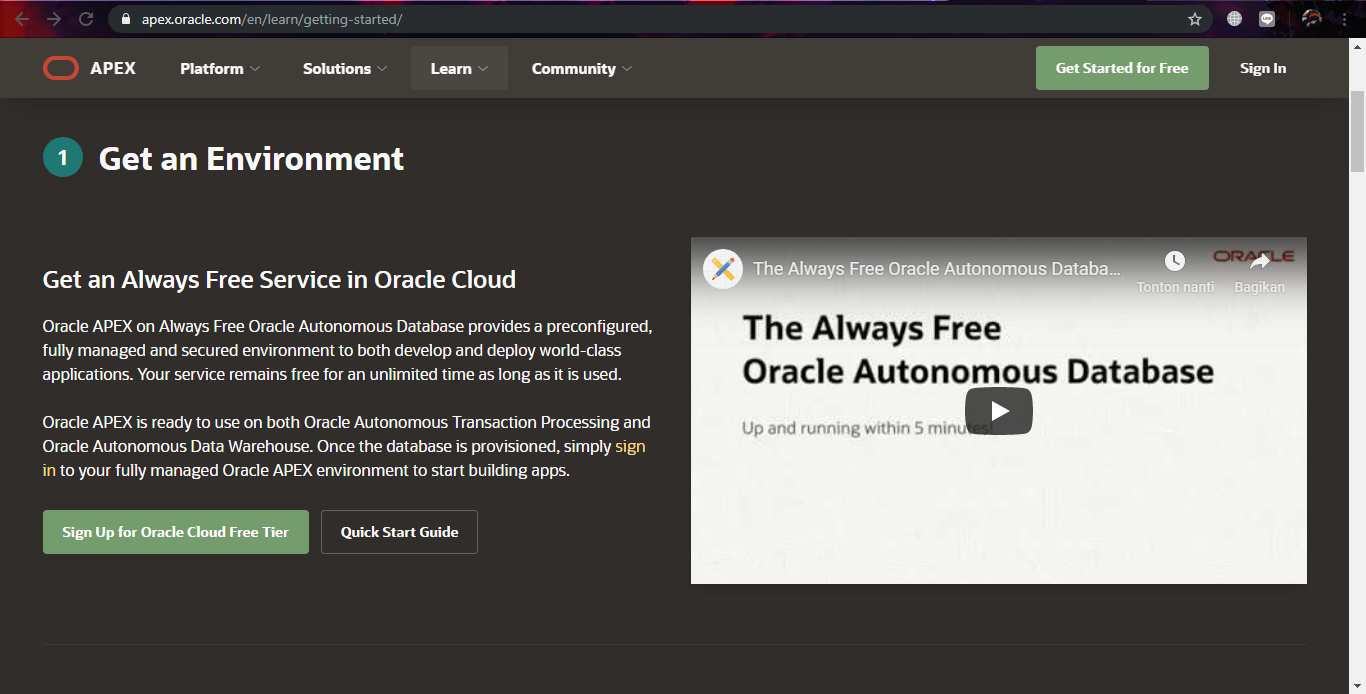
\includegraphics[scale=0.3]{1.PNG}
        \caption{Halaman Awal}
    \end{figure}
    \item Jika sudah maka langsung klik bagian \textit{request free workspace}
\newpage
    \item Jika sudah, maka akan masuk ke laman ini.
    \begin{figure}[!htbp]
        \centering
        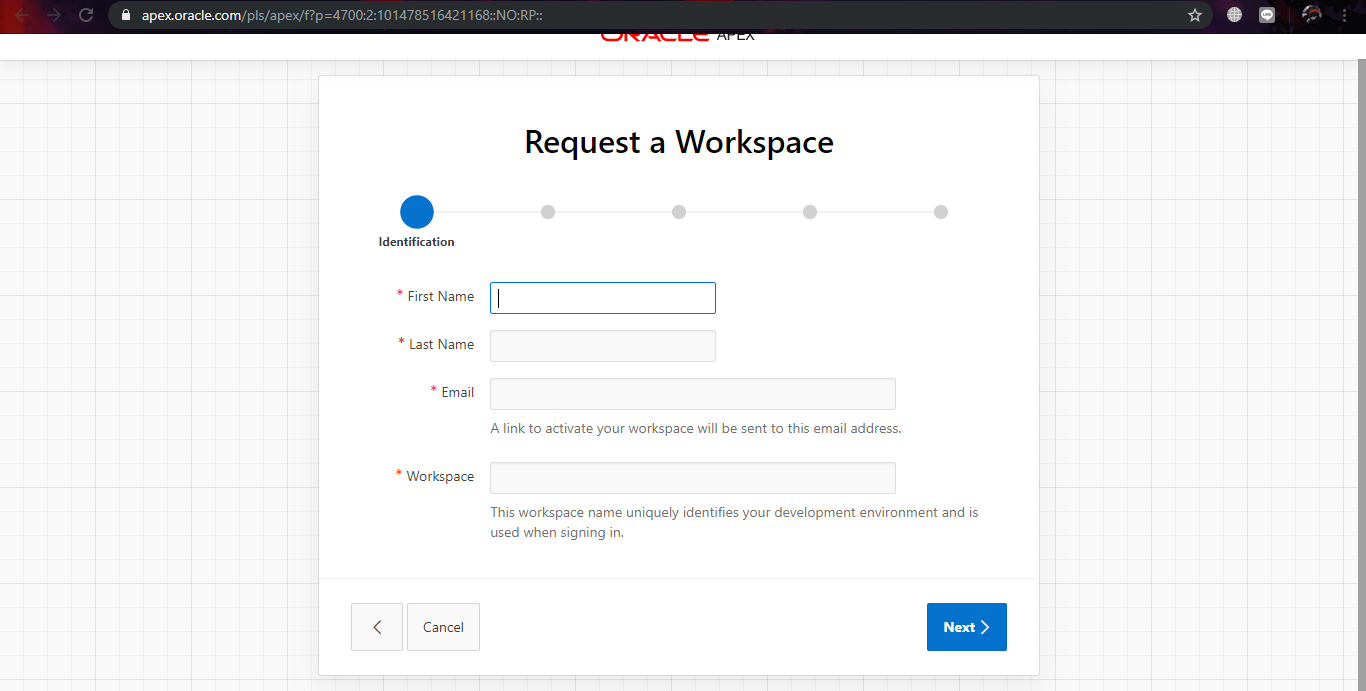
\includegraphics[scale=0.3]{2.PNG}
        \caption{Konfigurasi Workspace}
    \end{figure}
    \item Selanjutnya masukkan firstname, lastname dan yang lainnya sesuai dengan keinginan anda
    \item Jika sudah, langsung lanjut dan masuk ke halaman ini.
    \begin{figure}[!htbp]
        \centering
        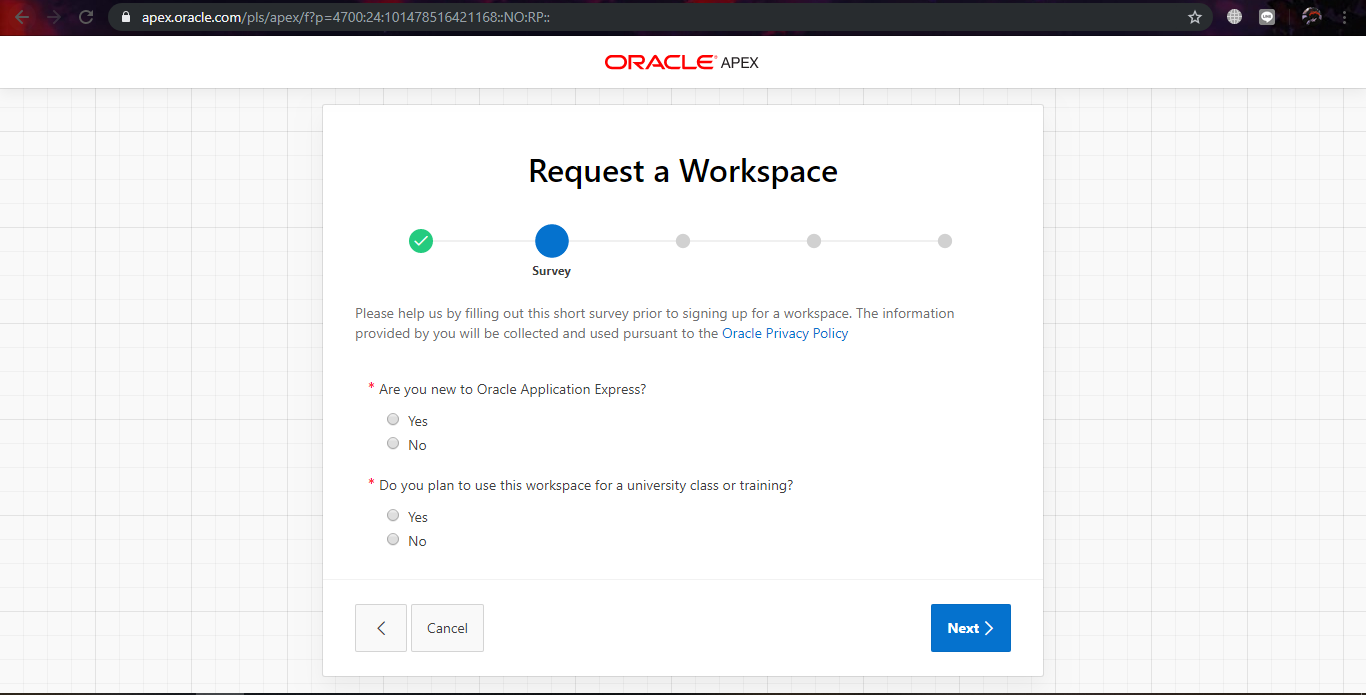
\includegraphics[scale=0.3]{3.PNG}
        \caption{Konfigursi Workspace(2)}
    \end{figure}
\newpage
    \item Pilih sesuai dengan keinginan anda.
    \item Selanjutnya klik next dan akan muncul tampilan seperti ini.
    \begin{figure}[!htbp]
        \centering
        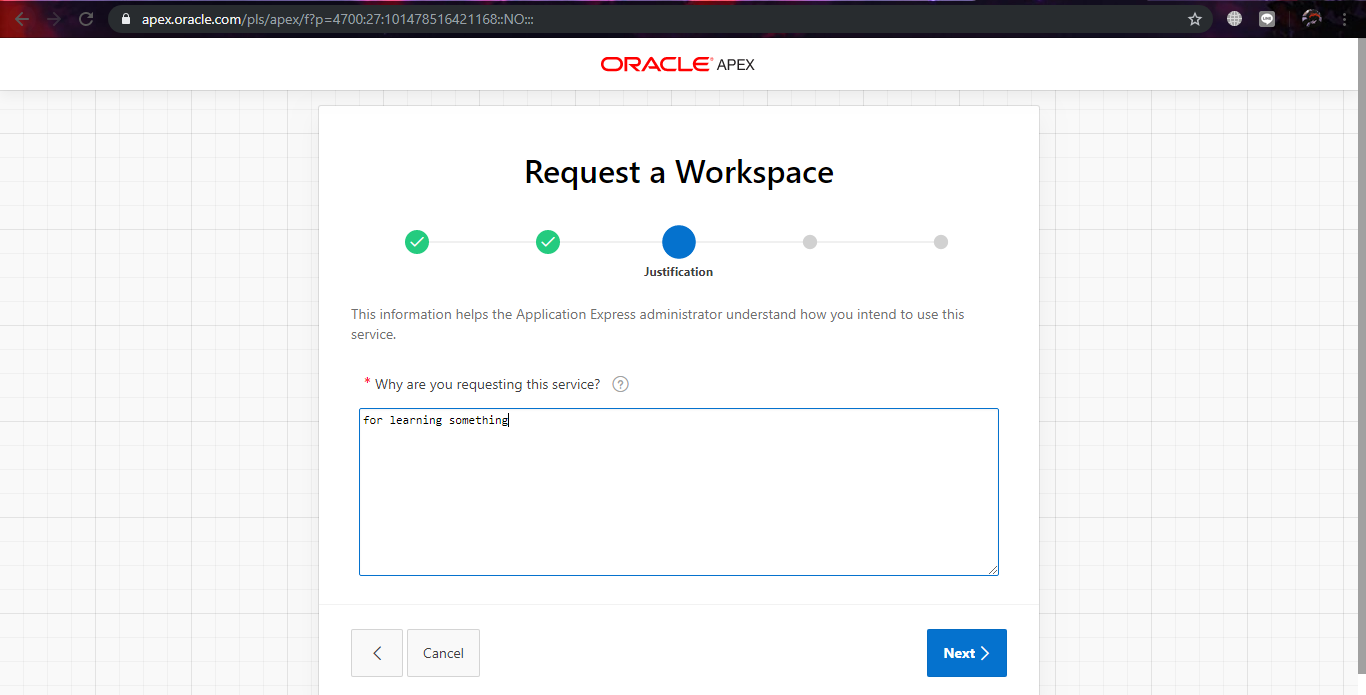
\includegraphics[scale=0.3]{4.PNG}
        \caption{Konfigurasi Workspace(3)}
    \end{figure}
    \item Isi sesuai keinginan kalian.
    \item Setelah itu klik next dan akan muncul tampilan seperti ini.
    \begin{figure}[!htbp]
        \centering
        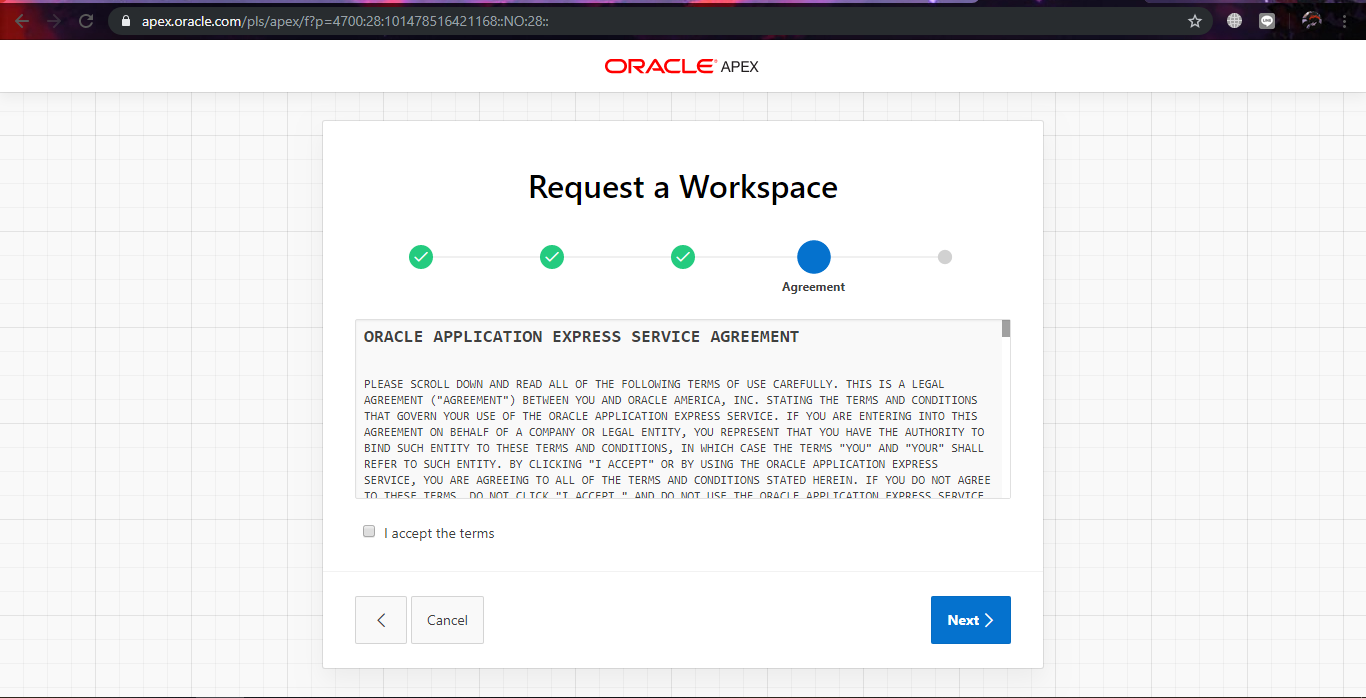
\includegraphics[scale=0.3]{5.PNG}
        \caption{Konfigurasi Workspace(4)}
    \end{figure}
\newpage
    \item Klik accept, dan next
    \item Seterusnya klik submit dan request dan akan muncul tampilan seperti ini
    \begin{figure}[!htbp]
        \centering
        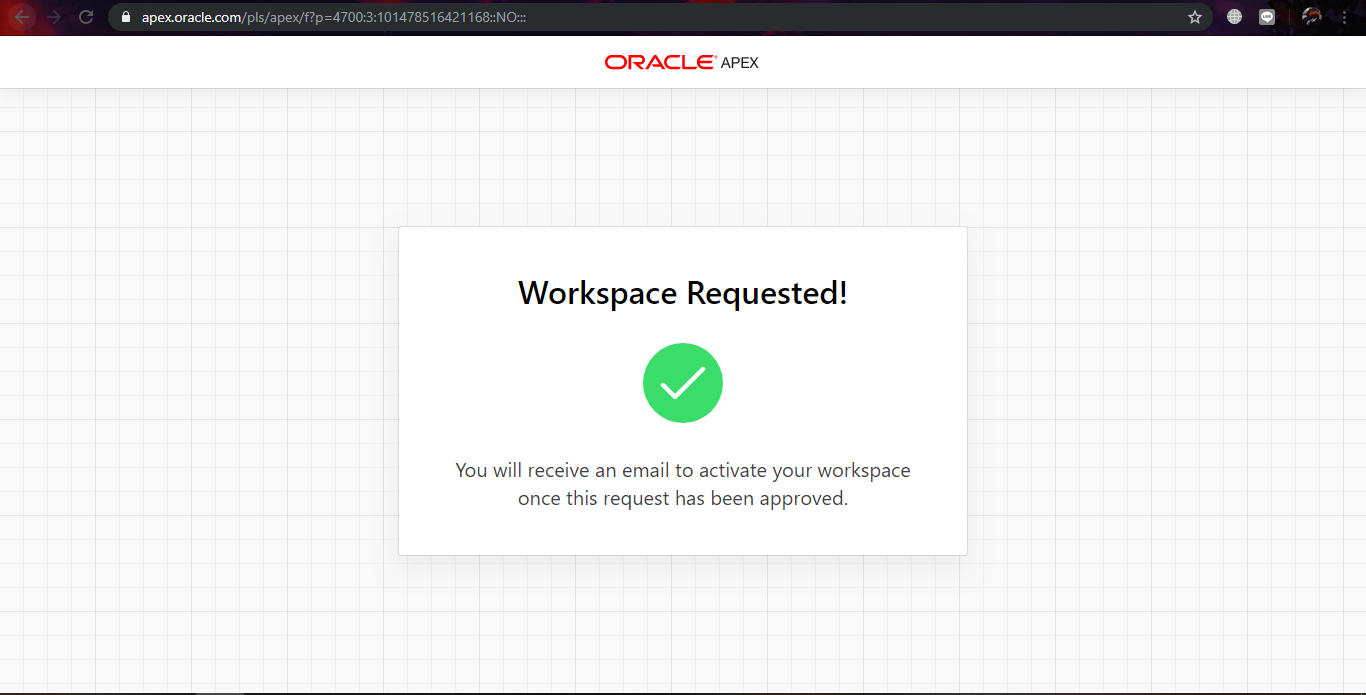
\includegraphics[scale=0.3]{6.PNG}
        \caption{Konfigurasi Workspace(5)}
    \end{figure}
    \item Kalian tinggal ngecek email dan mengaktifkan workspace tersebut
    \item Jika sudah di klik pada bagian email kalian, maka akan muncul pemberitahuan \textit{workspace successfully created}
    \begin{figure}[!htbp]
        \centering
        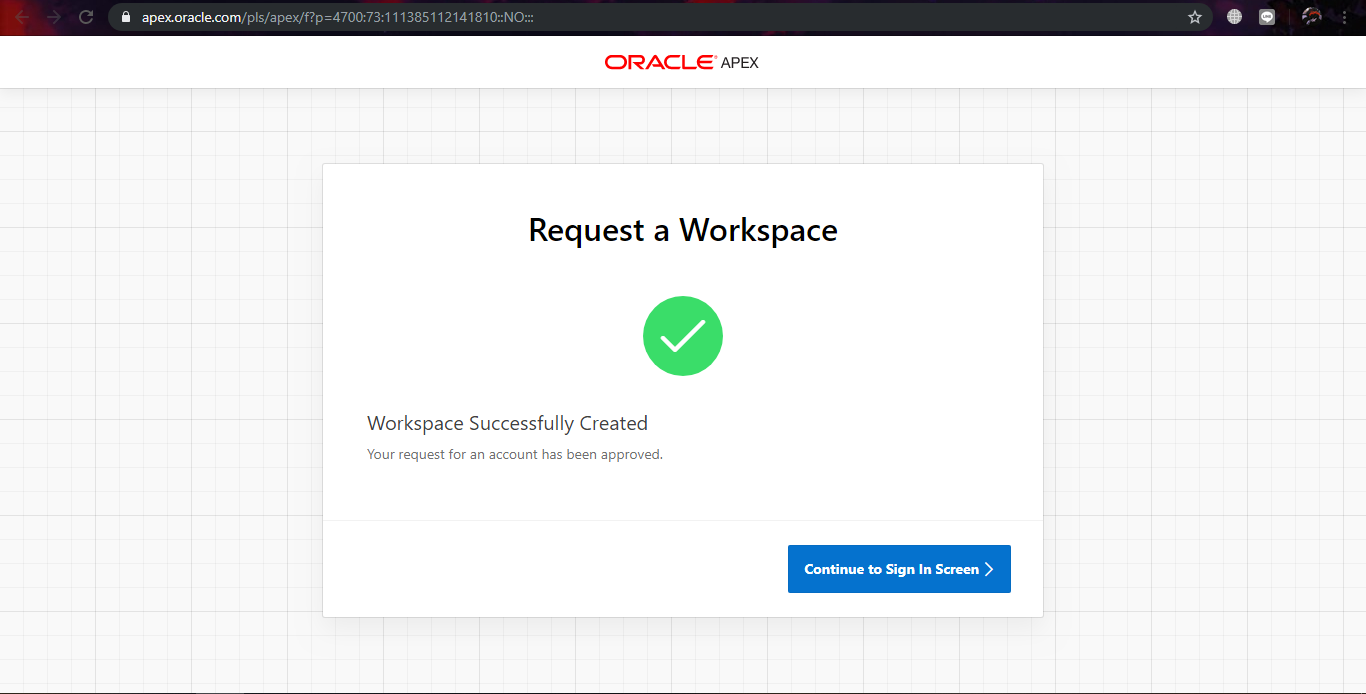
\includegraphics[scale=0.3]{7.PNG}
        \caption{Workspace telah dibuat}
    \end{figure}
\end{enumerate}
\newpage
\section{Membuat Aplikasi}
\begin{enumerate}
    \item Pertama, kalian akan login terlebih dahulu ketika sudah selesai membuat 
    \begin{figure}[!htbp]
        \centering
        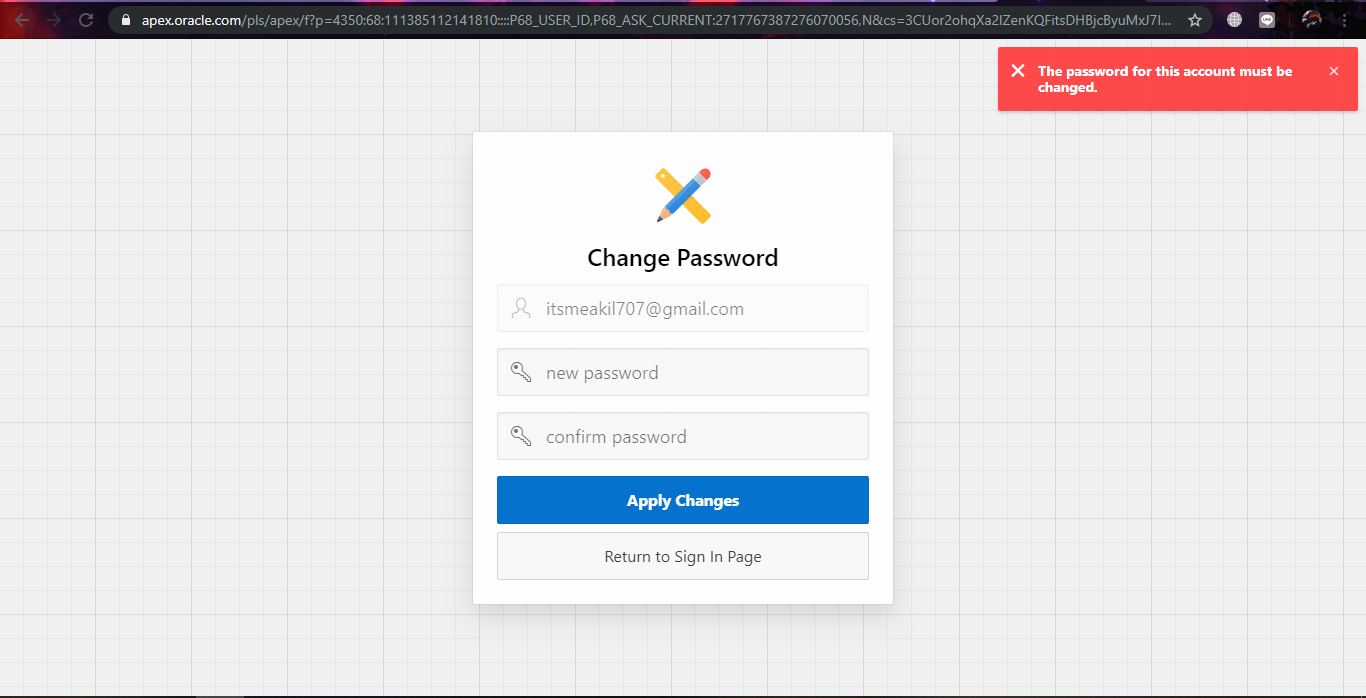
\includegraphics[scale=0.3]{8.PNG}
        \caption{Login}
    \end{figure}
    \item Ada pemberitahuan bahwa password harus diubah, maka password kalian ubah.
    \item Selanjutnya klik next maka akan masuk ke halaman utama apex.
    \begin{figure}[!htbp]
        \centering
        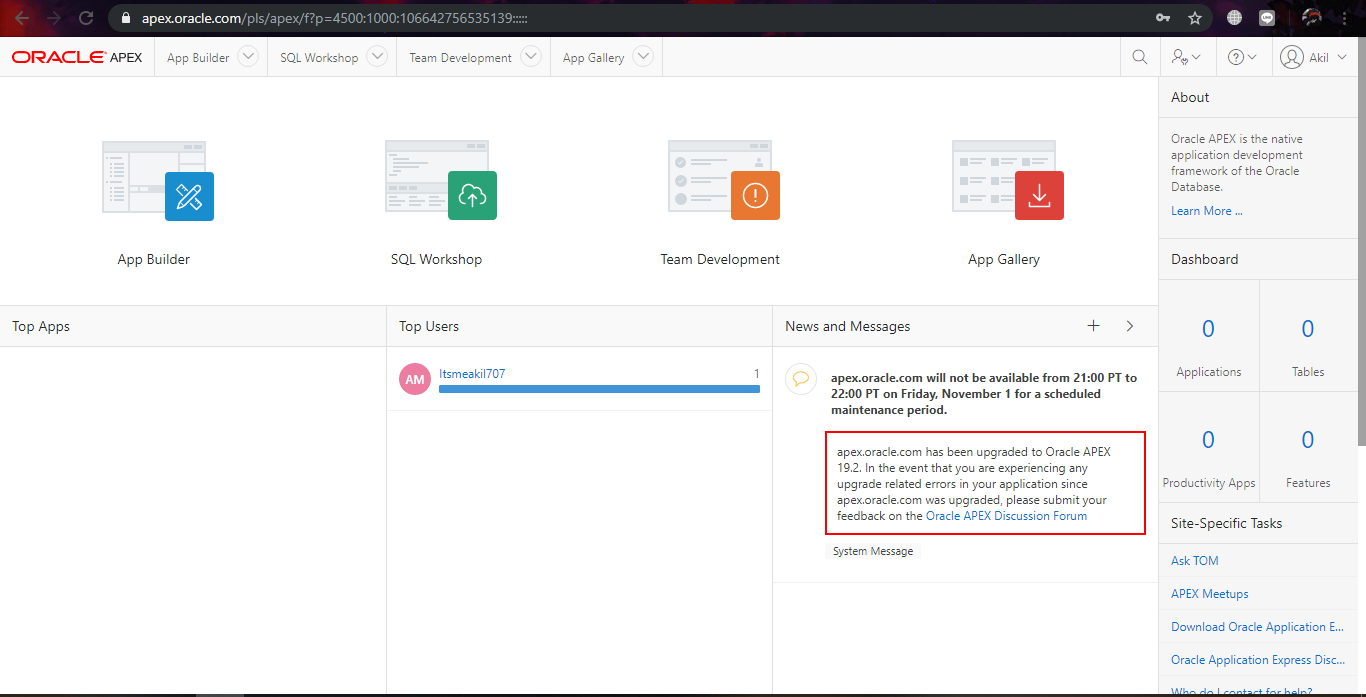
\includegraphics[scale=0.3]{9.PNG}
        \caption{Halaman Utama}
    \end{figure}
\newpage
    \item Setelah itu, klik bagian \textit{App Builder}
    \item Dan akan ada tampilan seperti ini
    \begin{figure}[!htbp]
        \centering
        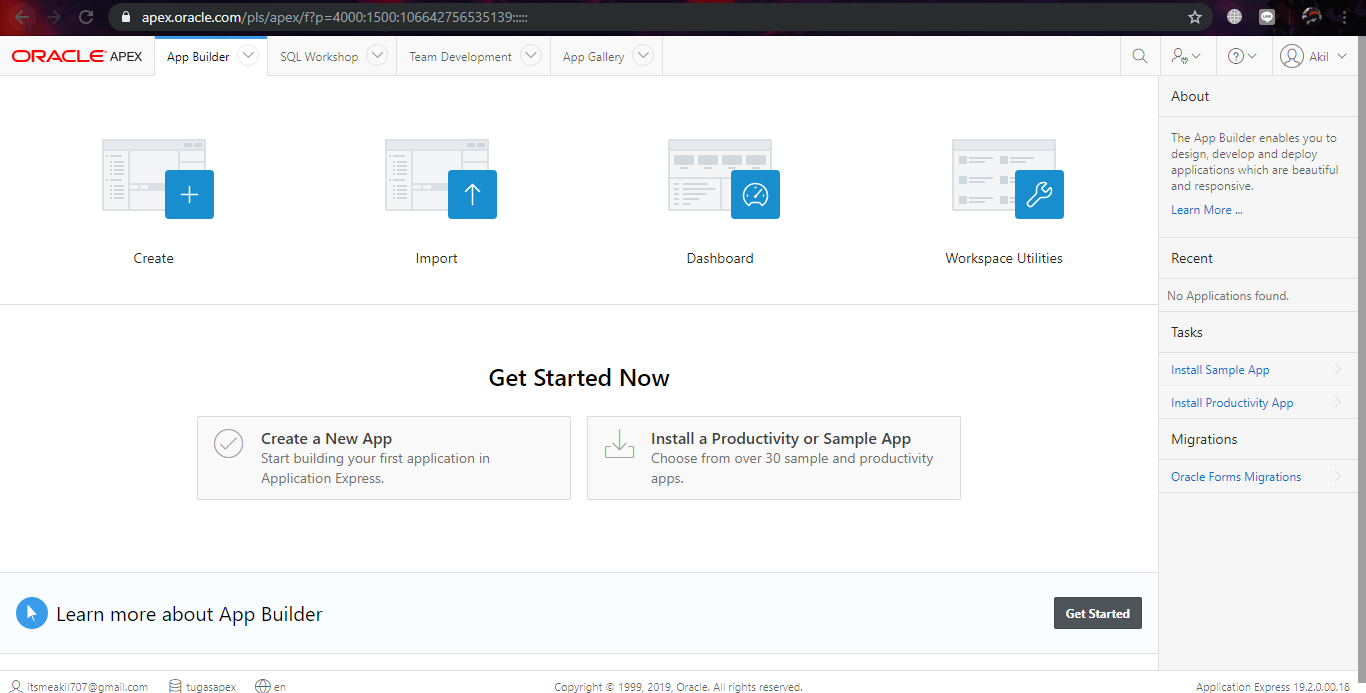
\includegraphics[scale=0.3]{10.PNG}
        \caption{Halaman App Builder}
    \end{figure}
    \item Setelah itu klik create dan akan ada tampilan seperti ini
    \begin{figure}[!htbp]
        \centering
        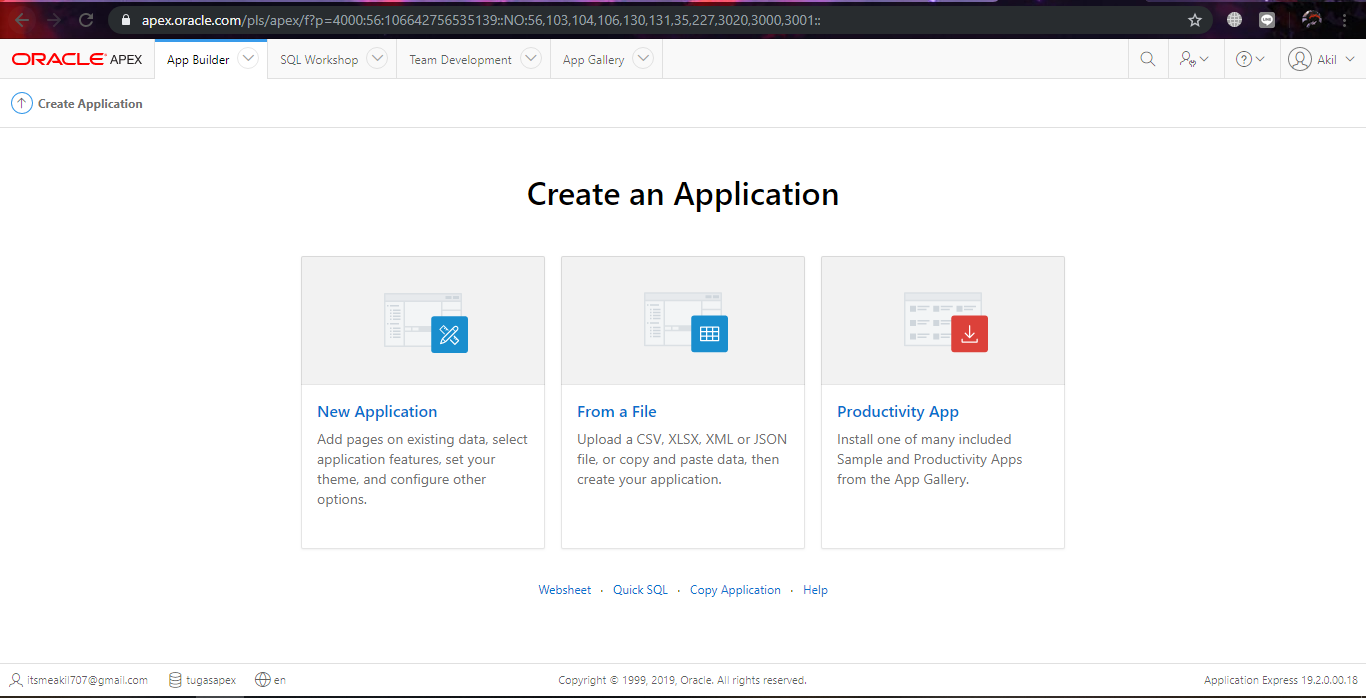
\includegraphics[scale=0.3]{11.PNG}
        \caption{Create Application}
    \end{figure}
    \item Pilih upload file
    \item Dan pilih file csv yang sudah kita sediakan
\newpage
    \item Disini saya sediakan 2 file yang nantinya akan kita relasikan
    \begin{figure}[!htbp]
        \centering
        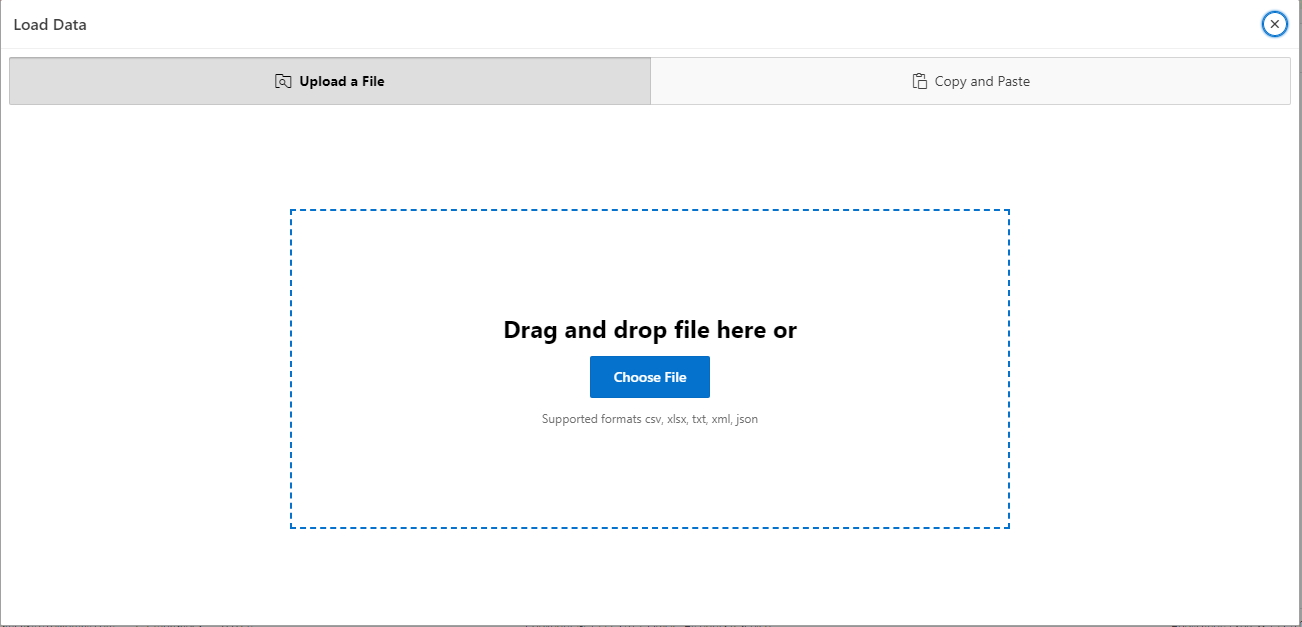
\includegraphics[scale=0.3]{12.PNG}
        \caption{Pilih file nya}
    \end{figure}
    \item Filenya ada angkatan mahasiswa, dan file alumni
    \begin{figure}[!htbp]
        \centering
        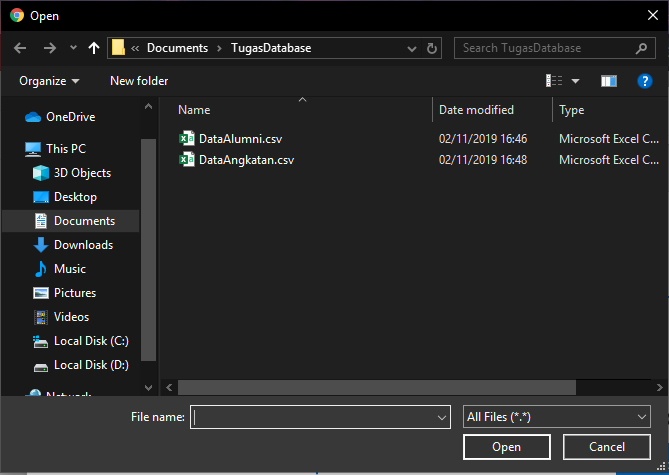
\includegraphics[scale=0.5]{13.PNG}
        \caption{Ada dua file}
    \end{figure}
\newpage
    \item Pilih file data angkatan dan konfigurasi seperti dibawah ini.
    \begin{figure}[!htbp]
        \centering
        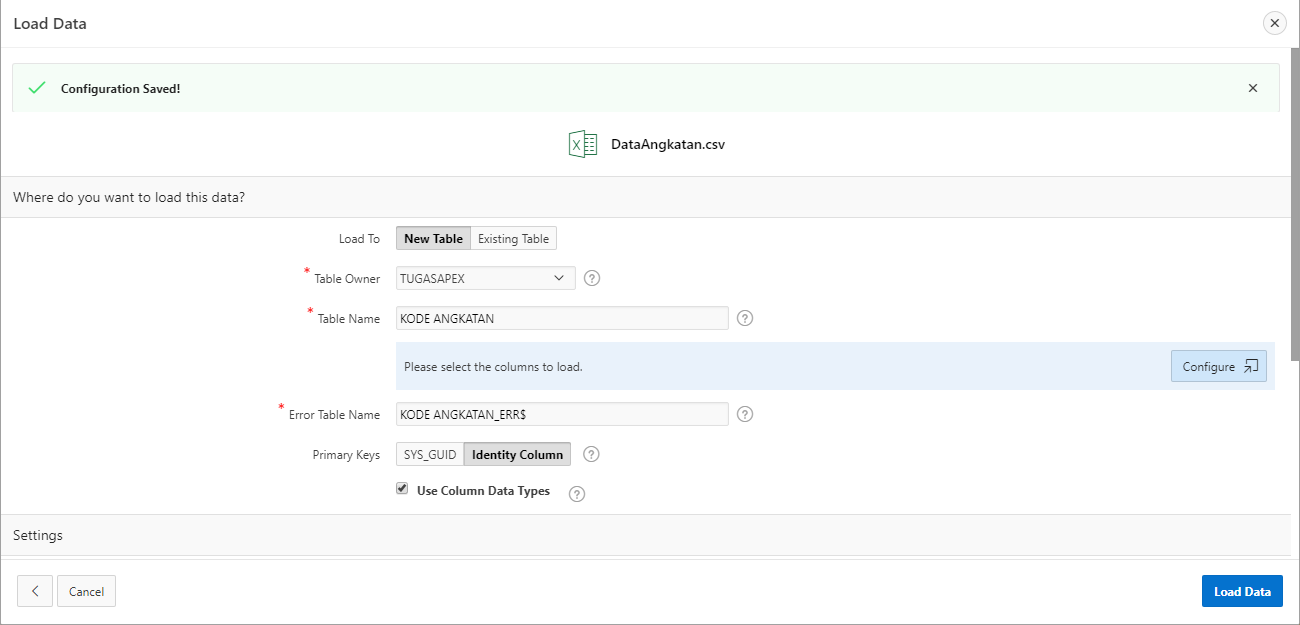
\includegraphics[scale=0.3]{14.PNG}
        \caption{Konfigurasi Data Angkatan}
    \end{figure}
    \item Sesudah itu klik load data, tapi jangan dilanjutkan dengan create application, namun langsung kita close, dan upload file data alumni sama seperti diatas dan konfigurasinya juga seperti itu.
    \begin{figure}[!htbp]
        \centering
        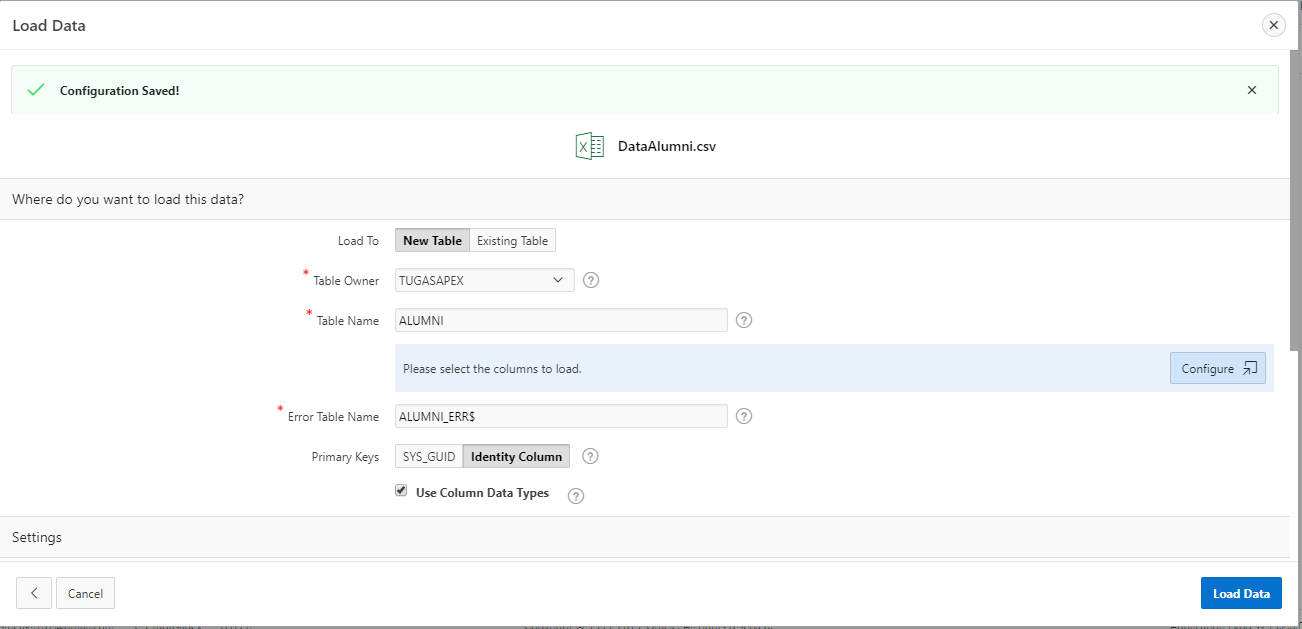
\includegraphics[scale=0.3]{15.PNG}
        \caption{Konfigurasi Data Alumni}
    \end{figure}
\newpage
    \item Sesudah itu kita klik create application
    \item Nanti akan tampil, tampilan seperti ini
    \begin{figure}[!htbp]
        \centering
        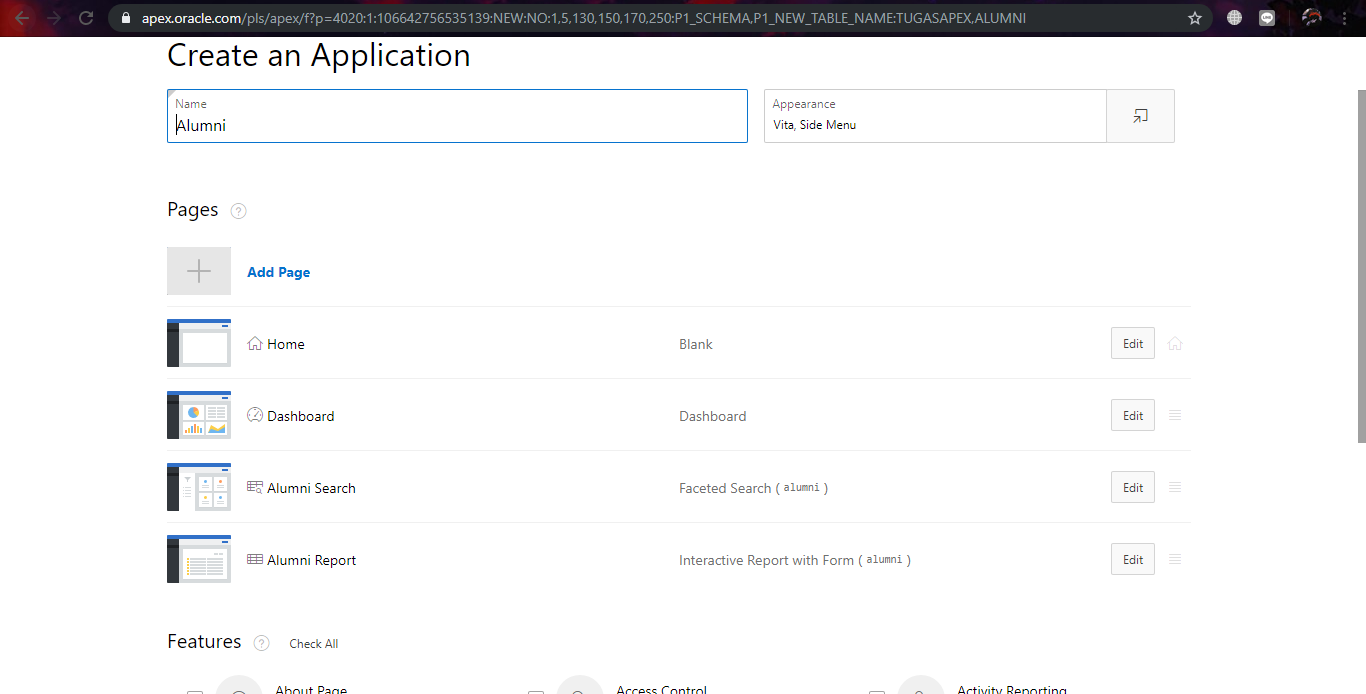
\includegraphics[scale=0.3]{17.PNG}
        \caption{Halaman Konfigurasi}
    \end{figure}
    \item Ketika sudah, maka menuju \textit{Alumni Report}, dan klik garis tiga disampingnya dan akan seperti ini.
    \begin{figure}[!htbp]
        \centering
        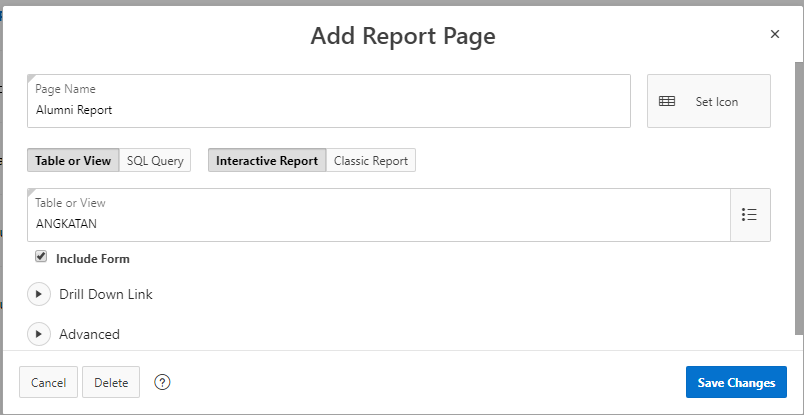
\includegraphics[scale=0.5]{18.PNG}
        \caption{Report Page}
    \end{figure}
    \item Jika sudah maka save changes
    \item Setelah itu, langsung klik \textit{create application}
\newpage
    \item Setelah itu, kita akan dihadapkan dengan halaman apex nya.
    \item Jika tidak ada lagi yang ingin di lakukan, maka klik run application untuk melihat aplikasi yang sudah jadi tadi.
    \begin{figure}[!htbp]
        \centering
        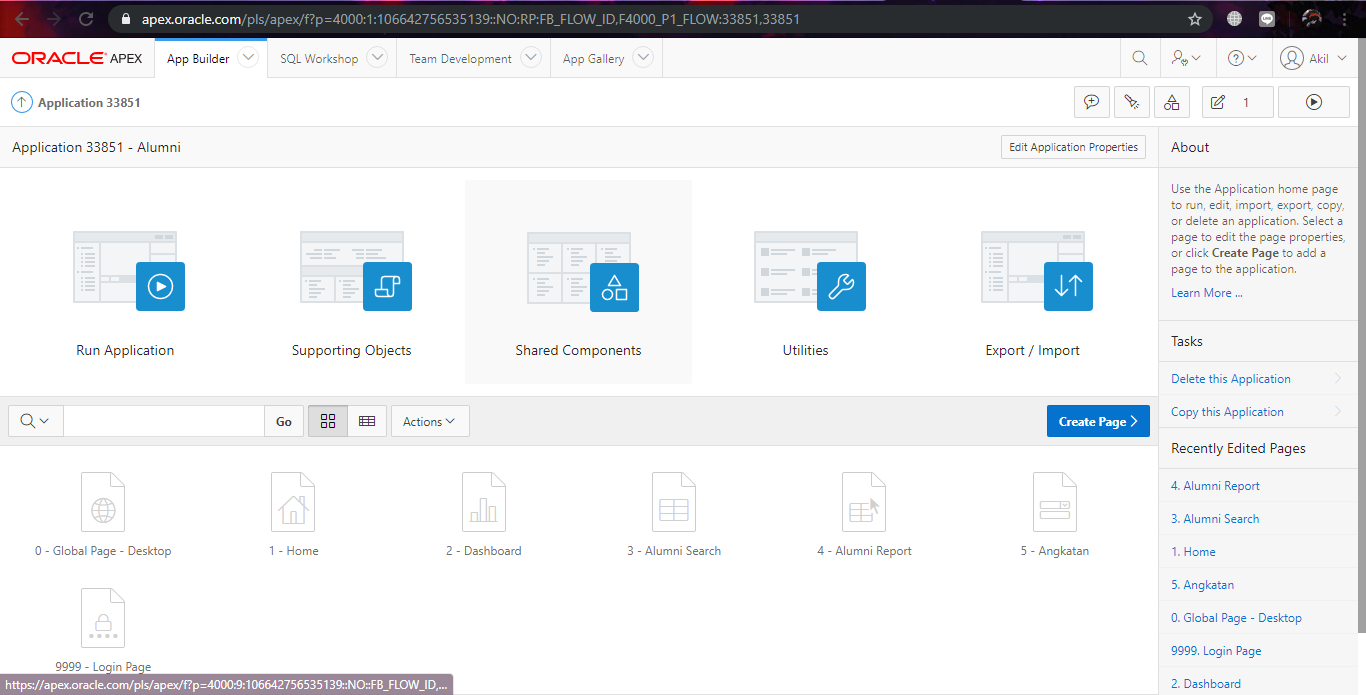
\includegraphics[scale=0.3]{20.PNG}
        \caption{Halaman Apex}
    \end{figure}
    \item Maka aplikasi yang sudah jadi akan seperti ini tampilannya
    \begin{figure}[!htbp]
        \centering
        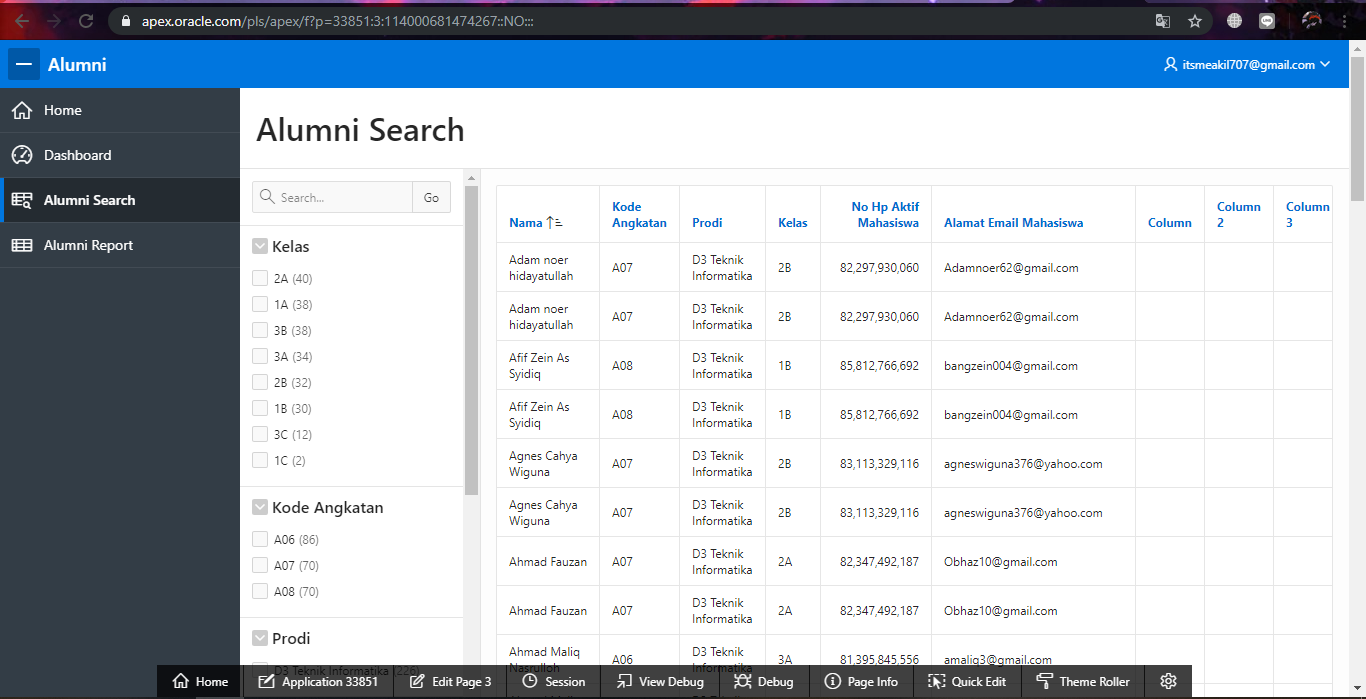
\includegraphics[scale=0.3]{21.PNG}
        \caption{Aplikasi Yang sudah jadi}
    \end{figure}
\newpage
    \item Berikut adalah pass dan username dari workspace saya
    \begin{figure}[!htbp]
        \centering
        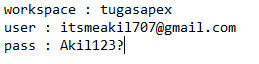
\includegraphics{userapex.PNG}
        \caption{User Apex}
    \end{figure}
    \item https://apex.oracle.com/pls/apex/f?p=4550:1:24850434092167:::::
\end{enumerate}

\end{document}
